\if0
☆レポート課題(チームで一部だけ提出して下さい)

1. 表紙(課題名、チームメンバ氏名、提出日)

2. SingleCycleMIPSのモジュール仕様書
 設計した各モジュールについて、上位階層から順に、下記の内容をまとめること。
 ・モジュール名
 ・モジュールの入出力信号名とその説明

例: 入力信号一覧
name 	width 	explanation
CLK 	[0:0] 	SingleCycleMIPS用クロック信号
PC 	[31:0] 	次に実行する命令アドレスを格納するレジスタ値


 ・モジュール内のブロック図(サブモジュール間の接続関係を明示すること。ただし、最下層のIF, ID, EX, MAについては、ブロック図は不要です。)
 ・モジュールの動作の説明文

3. 実機DE10-Liteでの動作検証
 ・テストプログラムのファイル名一覧(load_store, arithmetic, array, if_then_else, while, function, recursion, hanoi)
 ・テストプログラムの実行方法
 ・テストプログラムの検証法
 ・各テストプログラムの検証結果

4. 考察(メンバ一人づつ、個別の考察を記述して下さい。1600文字以上/人)
 ・今回の回路設計で工夫した点(技術的な視点、チーム内での役割分担等のプロジェクト管理的な視点)
 ・より実用的なMIPSプロセッサを実現するために、マイクロアーキテクチャの観点から改良すべき点、および、それに関連して追加で実装すべき機能/回路

5. 感想(メンバ一人づつ、個別の感想を記述して下さい。800文字程度)

6.参考文献
\fi
\documentclass[dvipdfmx]{jsarticle}
\usepackage{graphicx}[dvipdfmx]
\usepackage{multirow}
\usepackage{array}
\usepackage{amsmath,amssymb}
\usepackage{url}
\usepackage{listings}
\usepackage{color}
\usepackage{verbatim}

\title{計算機設計論 レポート課題:MIPSプロセッサの回路設計}
\author{1295149 森岡悠人\\}
\date{\today}

\begin{document}
\maketitle

\section{モジュール仕様書}


QuartusのRTL Viewerを用いて出力した,DE10-liteに書き込んだモジュールのブロック図を図\ref{fig:rtl}に示す.
\begin{figure}[h]
\centering
  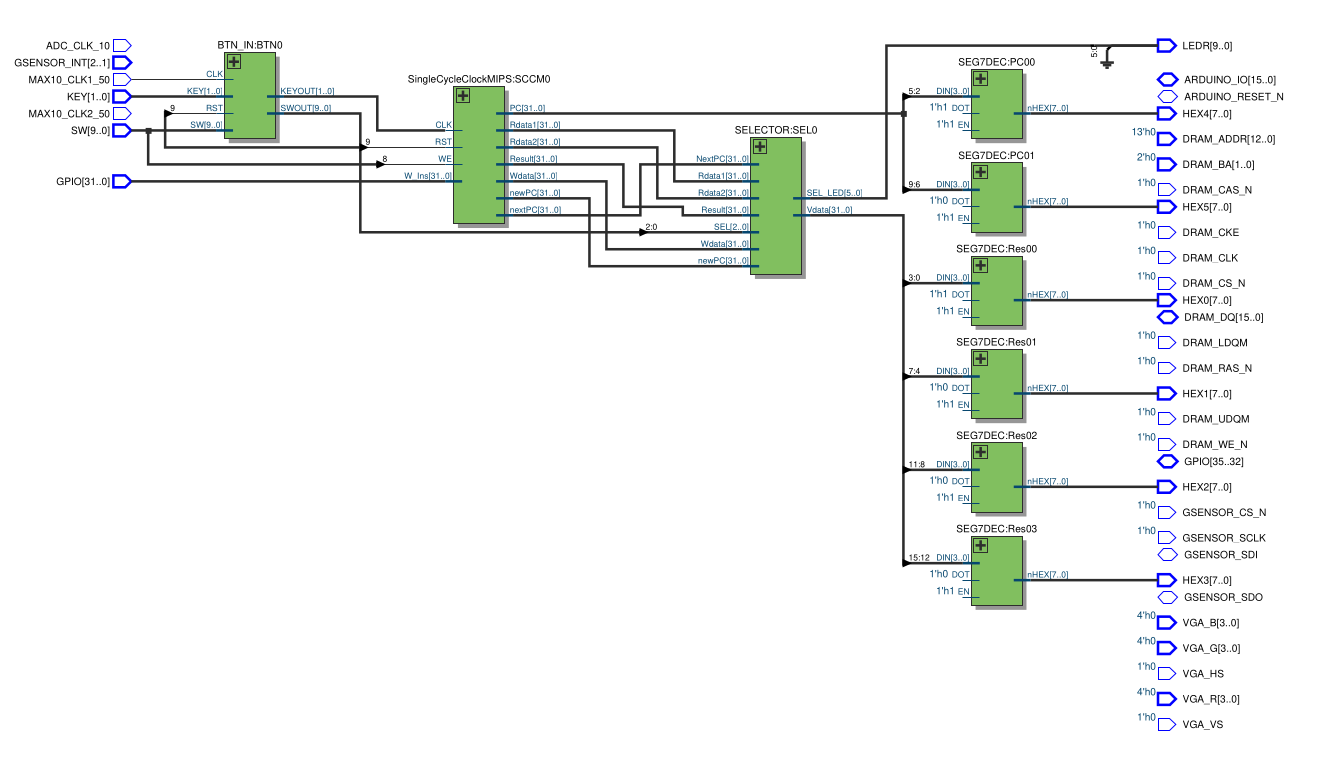
\includegraphics[width=\textwidth]{myRTL.png}
  \caption{作成したMIPS回路のブロック図}
  \label{fig:rtl}
\end{figure}



\section{動作検証}
作成したverilogコードがMIPSの命令セットを実行できるかどうかの検証を行った.
テストプログラムとして,教科書\cite{textbook}に掲載されているアセンブラプログラム(load\_store, arithmetic, array, if\_then\_else, while, function, recursion, hanoi)を用いた.
プログラムはCPUlator MIPS System Simulator \cite{mips-sim}を用いてコンパイルした.
その後32bitの16進数で出力されたバイナリを\texttt{IMem.txt}に書き込んでおき,IMに読み込ませた状態でシミュレーションを実行した.
動作の流れとデータメモリの中身を確認するため,modelsim20.1を用いて動作のシミュレーションと検証を行った.
シミュレーション結果は,display命令を用いて,PC, Instruction, ALU\_resultレジスタの順番が期待通りかどうかを確認した.
シミュレーションの様子を図\ref{fig:simulation}に示す.
\begin{figure}[h]
\centering
  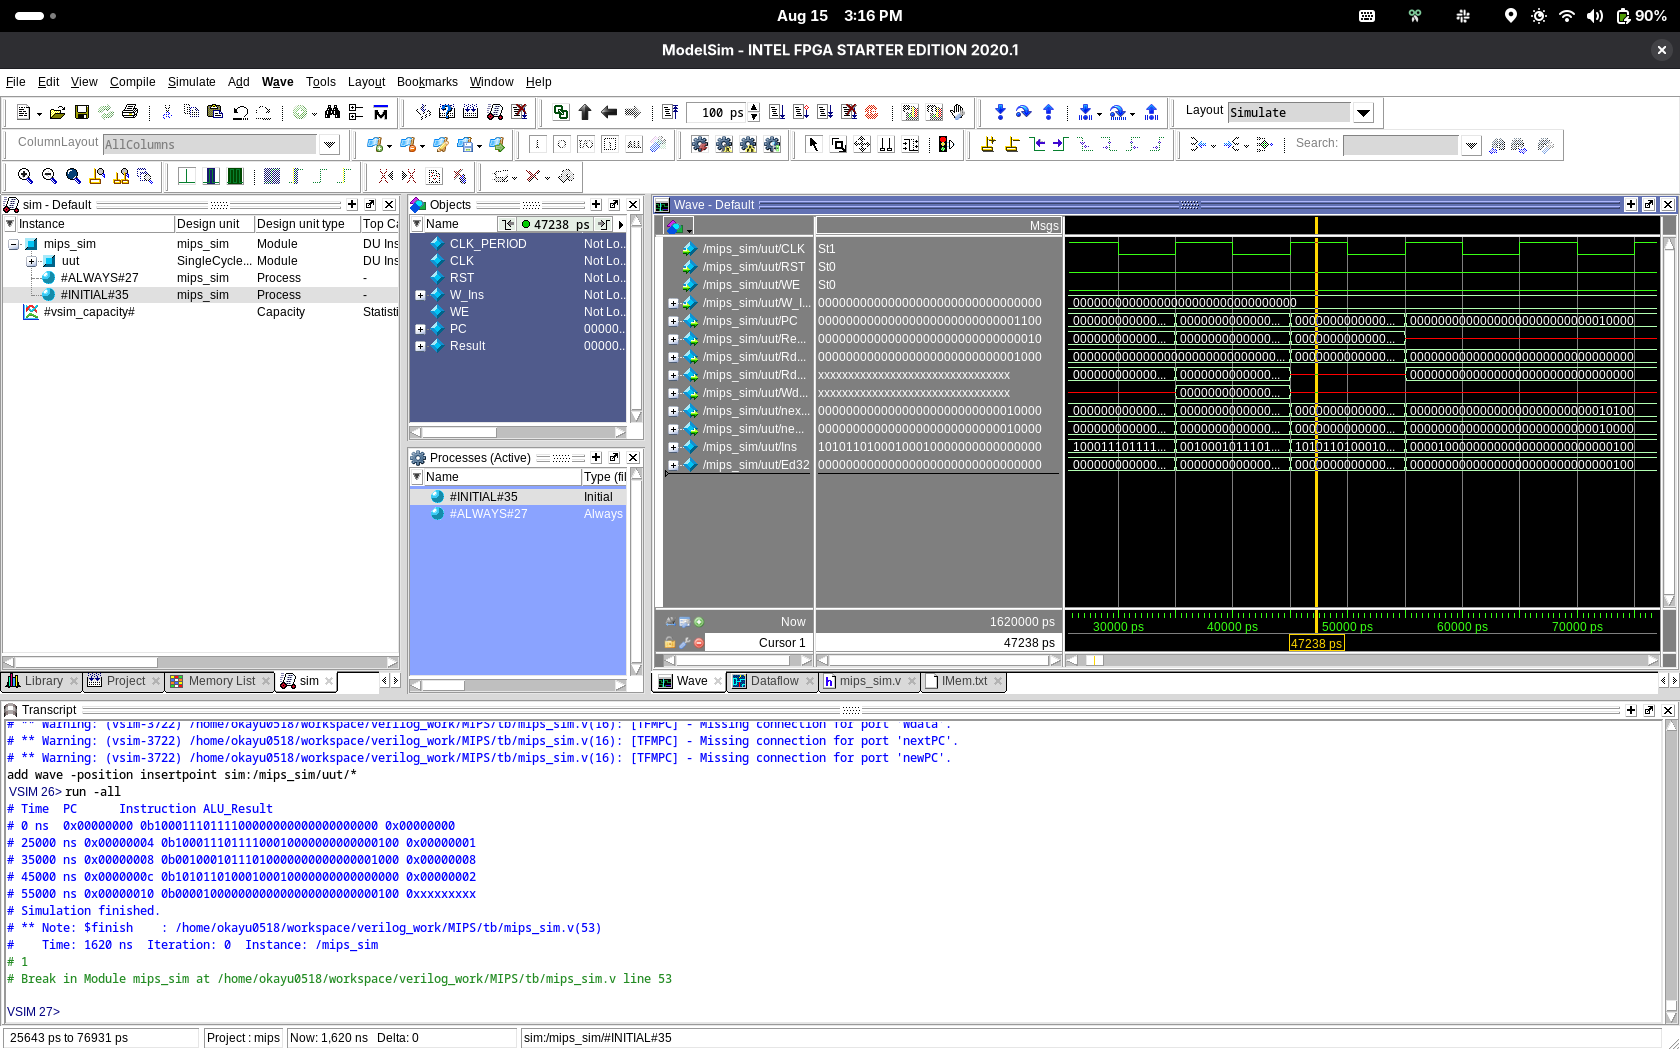
\includegraphics[width=0.8\textwidth]{modelsim.png}
  \caption{modelsimによるシミュレーションの様子}
  \label{fig:simulation}
\end{figure}

\subsection{test: load\_store}
基本的なロード・ストア命令の動作確認を行った.このプログラムではデータメモリから値をロードし、別のアドレスにストアする処理を行う.
プログラムの動作は以下の通りである:
\begin{itemize}
\item \texttt{lw \$s0, 0(\$s7)}: データメモリのアドレス\texttt{\$s7+0}から値をロードし、\texttt{\$s0}に格納
\item \texttt{lw \$s1, 4(\$s7)}: データメモリのアドレス\texttt{\$s7+4}から値をロードし、\texttt{\$s1}に格納  
\item \texttt{addi \$t0, \$s7, 8}: \texttt{\$s7+8}をアドレスとして\texttt{\$t0}に計算
\item \texttt{sw \$s1, 0(\$t0)}: \texttt{\$s1}の値を\texttt{\$t0}が示すアドレスにストア
\end{itemize}
あらかじめテストベンチでDMemの0番地からそれぞれ静的変数a=10,b=20と,配列a[0]=0,配列のオフセットを保持するレジスタ\$s7=0を初期値として設定してシミュレーションを実行した.
その結果,期待通り\$s0=10, \$s1=20, DMem[0]=10であることを確認した.
使用したアセンブリコードとそのテスト結果を付録\ref{appendix:load_store}に示す.

\subsection{test: arithmetic}
基本的な算術演算命令の動作を確認するためのテストを行った.このプログラムは3つの値を読み込んで加算を行い、結果をレジスタに格納する.
プログラムの動作は以下の通りである:
\begin{itemize}
\item 変数a, b, cの値(1, 2, 3)をそれぞれ\texttt{\$s0}, \texttt{\$s1}, \texttt{\$s2}にロード
\item \texttt{add \$t0, \$s0, \$s1}: a + b の結果を\texttt{\$t0}に格納
\item \texttt{add \$s3, \$t0, \$s2}: (a + b) + c の結果を\texttt{\$s3}に格納(期待値:6)
\end{itemize}
あらかじめテストベンチでDMemの0番地からそれぞれ静的変数a=1,b=2,c=3,d=0と変数のオフセットを保持するレジスタ\$s7=0を初期値として設定してシミュレーションを実行した.
その結果,期待通りa, b, cの値がadd命令で足し合わされ,\$s3=6であることを確認した.
使用したアセンブリコードとそのテスト結果を付録\ref{appendix:arithmetic}に示す.

\subsection{test: array}
配列のアクセスとインデックス計算の動作を確認するためのテストを行った.
プログラムの動作は以下の通りである:
\begin{itemize}
\item \texttt{sll \$t0, \$s0, 2}: インデックス\texttt{\$s0}を4倍(左シフト2ビット)してワードアドレスに変換
\item \texttt{add \$t0, \$s7, \$t0}: 配列の基底アドレス\texttt{\$s7}にオフセットを加算
\item \texttt{lw \$s1, 0(\$t0)}: 計算されたアドレスから配列要素をロード
\item \texttt{lw \$s2, 20(\$s7)}: 配列の5番目の要素(20バイトオフセット)をロード
\end{itemize}
あらかじめテストベンチでDMemの0番地からそれぞれ配列a[0]=0, a[1]=1, ..., a[9]=9と配列のオフセットを保持するレジスタ\$s7=0と\$s2=2を初期値として設定してシミュレーションを実行した.
その結果,期待通り\$s1=2, \$s2=5であることを確認した.
使用したアセンブリコードとそのテスト結果を付録\ref{appendix:array}に示す.

\subsection{test: if\_then\_else}
条件分岐命令の動作を確認するためのテストを行った.
プログラムの動作は以下の通りである:
\begin{itemize}
\item \texttt{beq \$s0, \$s1, L1}: \texttt{\$s0}と\texttt{\$s1}が等しい場合はL1にジャンプ
\item 等しくない場合:\texttt{\$s2 = \$s0}を実行してN1にジャンプ
\item 等しい場合(L1):\texttt{\$s2 = \$s1}を実行
\end{itemize}
まず,if文が真になる場合のテストを行った.
あらかじめテストベンチでレジスタ\$s0=0xa, \$s1=0xa, \$s2=0x0を初期値として設定してシミュレーションを実行した.
その結果,\$s0と\$s1が等しいため,\$s2に\$s1の値が代入され,\$s2=0xaであることを確認した.
次に,if文が偽になる場合のテストを行った.
あらかじめテストベンチでレジスタ\$s0=0xa, \$s1=0xb, \$s2=0x0を初期値として設定してシミュレーションを実行した.
その結果,\$s0と\$s1が等しくないため,\$s2に\$s0の値が代入され,\$s2=0xaであることを確認した.
真の場合と偽の場合のPCの遷移を比べると,偽の場合はelse節のラベルを飛び越えるためにJ命令が実行されているためことがわかる.
そのため偽の場合は1命令多い.使用したアセンブリコードとそのテスト結果を付録\ref{appendix:if_then_else}に示す.

\subsection{test: while}
ループ処理と条件判定の動作を確認するためのテストを行った.
プログラムの動作は以下の通りである:
\begin{itemize}
\item \texttt{slti \$t0, \$s0, 10}: \texttt{\$s0 < 10}の条件判定結果を\texttt{\$t0}に格納
\item 条件が偽(\texttt{\$s0 >= 10})の場合はループを終了してN1にジャンプ
\item 条件が真の場合:配列に\texttt{\$s0}の値を格納し、\texttt{\$s0}をインクリメントしてループを継続
\end{itemize}
あらかじめテストベンチで配列a[10]を0で初期化し,配列のオフセットを保持するレジスタ\$s7=0, \$s0=0を初期値として設定してシミュレーションを実行した.
その結果,\$s0が10になるまでwhile文が繰り返され,配列a[0]からa[9]にそれぞれ0から9までの値が代入されていることを確認した.使用したアセンブリコードとそのテスト結果を付録\ref{appendix:while}に示す.

\subsection{test: function}
\label{sec:function}
関数呼び出しとスタック操作の動作を確認するためのテストを行った.このプログラムは1からnまでの和を計算する関数を実装している.
プログラムの動作は以下の通りである:
\begin{itemize}
\item メイン部分:引数を\texttt{\$a0}に設定してsum関数を呼び出し、戻り値を\texttt{\$s1}に格納
\item sum関数:スタックにレジスタを退避し、1からnまでの和を計算して\texttt{\$v0}に結果を返す
\item 関数終了時にはスタックからレジスタを復元し、呼び出し元に戻る
\end{itemize}
あらかじめテストベンチでレジスタ\$s0=10を初期値として設定して1からnまでの和を求めるプログラムのシミュレーションを実行した.
その結果,\$s1=0x37=0d55となることを確認した.使用したアセンブリコードとそのテスト結果を付録\ref{appendix:function}に示す.

\subsection{test: recursion}
再帰関数呼び出しの動作を確認するためのテストを行った.このプログラムは再帰を用いて1からnまでの和を計算する.
プログラムの動作は以下の通りである:
\begin{itemize}
\item 引数が1未満の場合は0を返してベースケースとする
\item 引数が1以上の場合は、引数を1減らして再帰呼び出しを行い、その結果に現在の引数値を加算
\item 各再帰レベルでスタックに引数と戻りアドレスを保存・復元
\end{itemize}
\ref{sec:function}のテストと同様に,あらかじめテストベンチでレジスタ\$s0=10を初期値として設定してシミュレーションを実行した.
その結果,\$s1=0x37=0d55となることを確認した.使用したアセンブリコードとそのテスト結果を付録\ref{appendix:recursion}に示す.

\subsection{test: hanoi}
ハノイの塔を解く再帰アルゴリズムを実装し、複雑な再帰処理の動作を確認するためのテストを行った.
プログラムの動作は以下の通りである:
\begin{itemize}
\item 3枚の円盤のハノイの塔問題を解く
\item \texttt{\$a0}: 円盤の枚数、\texttt{\$a1}: 移動元、\texttt{\$a2}: 移動先、\texttt{\$a3}: 補助杆
\item \texttt{\$t1}: 移動回数カウンタ(期待値:7回)
\item 再帰の深さに応じてスタックに多くの引数と戻りアドレスを保存
\item ベースケース(円盤が1枚)では直接移動を実行
\end{itemize}
円盤が3枚のハノイの塔を解くプログラムを実行する.
レジスタ\$t1を移動回数カウント用としてシミュレーションを行った.
結果,\$t1=7となり,期待通りの動作を確認した.
hanoiのテストは算術演算,関数呼び出しなど,上記の多くの処理を含むため,Quartus Primeを用いてDE10-Liteに書き込んで実行した.
その結果,modelsim同様に期待通りの動作をし,最後の無限ループの処理まで到達することを確認できた.使用したアセンブリコードとそのテスト結果を付録\ref{appendix:hanoi}に示す.



\section{考察}
\subsection{森岡悠人}
今回のMIPS回路設計の課題は松本と協力して課題を分担して取り組んだ.
定期的に対面で集まって作業し,問題点やバグを共有しながら進めた.
どうしても理解できない部分や,詰まった部分は岩田研究室のM1に聞きに行くことで解決した.
githubのリポジトリ上で共同編集を行ったが,回路のソースとテストベンチを分けて開発したため,変更が競合しづらく,効率よく開発を進めることができた.
私は作成した回路のテストを担当した.
まず,EX.vのテストベンチを書いて各命令を入力したときのALUのresultをチェックし,その後,MIPS全体のテストベンチを書いて教科書にあるテストプログラムを使って命令実行時の挙動を確認した.
テストベンチを作成する際,modelsimのwaveだけでは確認するときの効率が悪かったため,display命令を用いてテスト内容と結果はすべてコンソールに出力させた.
また,テスト内容について,生成AIを用いて効率よくテストを作成することを検討したが,生成AIはverilogの知識はあまりない様子で,生成したテスト内容はところどころミスがあり,結局すべてのテストを手動で確認して修正した.
しかし,テストベンチ全体の構造は生成AIを用いて作成したため,ある程度効率的にテストベンチを作成できた.
このとき,Instructionの値は,微妙な間隔でビットの区切りがあるため,バイナリで書いた.
さらに,命令の形式に対応したビットの区切りとなる箇所にはアンダーバーを入れて記述することで読みやすくなるように工夫した.
EX.vのテストベンチ全体として,\texttt{test\_instruction}というtaskを作成し,そこに各命令のテストとなる入力と期待する出力を入れ,比較することでテストを行った.
回路をデバッグする中で意識したことは,回路の出力が期待通りにならないとき,信号の流れを一つずつ追うことである.
modelsimのシミュレーションのみたい箇所の信号が確認できる機能を使って,どの信号線まで正常に信号が流れているかを入力から順番に確認することで,問題を特定できた.
また,modelsimのデータメモリの中身を確認する機能もsw命令のデバッグで非常に役に立った.
ただし,Online MIPS Simulatorでは.data領域に確保するメモリサイズや初期値をを記述すればコンパイルするときに勝手にメモリ上に配置してくれたのに対し,作成したMIPSではその機能がないため,テストベンチで手動でデータメモリの初期値を設定する必要があった.
これは大変だと感じ,既存のコンパイラやアセンブラの自動でメモリに初期値を書き込んでくれる機能のありがたみを感じた.
ただし,データメモリに初期値を書き込んだりするのは回路設計の果たして回路レベルでやるべき処理なのか疑問に思った.

今回作成したMIPSの改善点について述べる.
まず,FPGAボードの7セグに常にPCをワード単位で表示させたが,これはバイト単位の表示のほうが他シミュレータの結果との比較がしやすいのではないかと考える.
また,今回はIMem.txtにバイナリを書き込んでおき,それを読み込む形で命令を実行したが,テストベンチからIMに読み込ませるテキストファイルを指定できるようにできれば,あらかじめテストプログラムをファイル単位で用意しておいて実行できて,テストが捗るのではないかと考えた.
しかしそれはそれで,modelsimにもquartusにもIMem.txtを読み込む処理を別々に書かないといけないため,面倒だなと思った.
また,教科書のテストプログラムについて,MULTやDIVなど,実装したすべての命令が網羅できているとは言えず,\texttt{common_param.vh}のすべての命令をテストしようと思うと別で大量のテストベンチを書く必要がある.
そのため,もう少し網羅的かつ統一的にテストできるテストプログラムの雛形と正解となる出力データを先生側で用意してもらえるとテストも効率的に行えて,課題の確認もスムーズに行えて良いのではないかと思った.
また,講義内でテストベンチの作り方について説明が少なかったように感じられた.せめて,1命令のテスト分,また,display命令の使い方については説明してくれたほうがいいのではないかと考える.
今回のMIPSは教科書に従ってSE/UEや,MUXも全てassign文で実装した.
そのため,流れが追いやすく,デバッグしやすかった反面,他にも実装パターンは複数考えられるので,本当はさらに効率のいい実装方法があるのだろうなと思った.
それとも,コンパイルして論理合成すると,結局同じ回路になるのかどうか興味が湧いた.





\section{感想}
\subsection{森岡悠人}
この講義で初めてVerilogやFPGA開発を経験したが,これまでプログラミング言語しか触れてこなかったため,verilogの独自の命令やmoduleの考え方,並列で回路の処理が実行される考え方は新鮮で面白かった.
実際にFPGAが動作したときは達成感を感じた.
一方,初めてのHDLで,面食らったことも多々あった.
modelsimおよびquartus primeの操作やプロジェクトファイルの構造が独特で,かつ頻繁に強制終了するため,実装に非常に時間がかかった.
シミュレーションで,メモリの中身を見る機能や,回路のwaveを確認する画面で,自由にソースコードの信号を追加して確認できる機能は非常に便利だった.
だが,門屋に教えてもらうまではその存在に気が付かなかったため,もうちょっとわかりやすいUIにしてほしいと思った.
ハードウェアを設計する技術者の使うツールだから,そのために用いるソフトウェアもあまり出来が良くないのではないかと思った.
また,私が普段利用するChatGPTのようなAIは,おそらくVerilogのコード生成に必要な学習データが不足していて,間違ったコードを生成することが多く,あまり役に立たなかった.
また,1時間計からMIPSに取り掛かるときにレベルが一気に3段階くらい上がるなという印象を受けた.

私は将来は低レベルのコンピュータの動作を理解したエンジニアを目指しているため,この講義を受講した.
その結果,かつて苦しんだアセンブラの実験の内容をおさらいできたことに加え,FPGA実機を用いたverilogの回路設計の経験を積むことができ,新たな知見を得られたため,受講して良かったと感じている.
また,ペアの松本の実装が速く,常に私に先行してALUや命令実行時の動作について教えてくれた.
起こった問題に対して二人でアイデアを出し合いながら原因を検討し,試行錯誤の中で回路の理解を深められたことが,今回の課題がうまく行った理由ではないかと感じている.

\section*{謝辞}
本課題に取り組む過程で,忙しい中何度も有益な助言をくださった大崎綾斗さん,門屋陽丈さんに感謝いたします.

\appendix
\section{テストプログラム}

本節では、各テストプログラムのアセンブリコードとその動作、および実行結果について説明する。

\subsection{load\_store}
\label{appendix:load_store}

\subsubsection{プログラム}
このプログラムは基本的なロード・ストア命令の動作を確認するためのテストである。
プログラムでは、データメモリから値をロードし、別のアドレスにストアする処理を行う。

\verbatiminput{test-results/load_store.asm}

\textbf{プログラムの動作:}
\begin{itemize}
\item \texttt{lw \$s0, 0(\$s7)}: データメモリのアドレス\texttt{\$s7+0}から値をロードし、\texttt{\$s0}に格納
\item \texttt{lw \$s1, 4(\$s7)}: データメモリのアドレス\texttt{\$s7+4}から値をロードし、\texttt{\$s1}に格納  
\item \texttt{addi \$t0, \$s7, 8}: \texttt{\$s7+8}をアドレスとして\texttt{\$t0}に計算
\item \texttt{sw \$s1, 0(\$t0)}: \texttt{\$s1}の値を\texttt{\$t0}が示すアドレスにストア
\end{itemize}

\subsubsection{テスト結果}
\verbatiminput{test-results/load_store.txt}

\subsection{arithmetic}
\label{appendix:arithmetic}

\subsubsection{プログラム}
このプログラムは基本的な算術演算命令の動作を確認するためのテストである。
3つの値を読み込んで加算を行い、結果をレジスタに格納する。

\verbatiminput{test-results/arithmetic.asm}

\textbf{プログラムの動作:}
\begin{itemize}
\item 変数a, b, cの値(1, 2, 3)をそれぞれ\texttt{\$s0}, \texttt{\$s1}, \texttt{\$s2}にロード
\item \texttt{add \$t0, \$s0, \$s1}: a + b の結果を\texttt{\$t0}に格納
\item \texttt{add \$s3, \$t0, \$s2}: (a + b) + c の結果を\texttt{\$s3}に格納(期待値:6)
\end{itemize}

\subsubsection{テスト結果}
\verbatiminput{test-results/arithmetic.txt}

\subsection{array}
\label{appendix:array}

\subsubsection{プログラム}
このプログラムは配列のアクセスとインデックス計算の動作を確認するためのテストである。

\verbatiminput{test-results/array.asm}

\textbf{プログラムの動作:}
\begin{itemize}
\item \texttt{sll \$t0, \$s0, 2}: インデックス\texttt{\$s0}を4倍(左シフト2ビット)してワードアドレスに変換
\item \texttt{add \$t0, \$s7, \$t0}: 配列の基底アドレス\texttt{\$s7}にオフセットを加算
\item \texttt{lw \$s1, 0(\$t0)}: 計算されたアドレスから配列要素をロード
\item \texttt{lw \$s2, 20(\$s7)}: 配列の5番目の要素(20バイトオフセット)をロード
\end{itemize}

\subsubsection{テスト結果}
\verbatiminput{test-results/array.txt}

\subsection{if\_then\_else}
\label{appendix:if_then_else}

\subsubsection{プログラム}
このプログラムは条件分岐命令の動作を確認するためのテストである。

\verbatiminput{test-results/if_then_else.asm}

\textbf{プログラムの動作:}
\begin{itemize}
\item \texttt{beq \$s0, \$s1, L1}: \texttt{\$s0}と\texttt{\$s1}が等しい場合はL1にジャンプ
\item 等しくない場合:\texttt{\$s2 = \$s0}を実行してN1にジャンプ
\item 等しい場合(L1):\texttt{\$s2 = \$s1}を実行
\end{itemize}

\subsubsection{テスト結果(真の場合)}
\verbatiminput{test-results/if_then_else_true.txt}

\subsubsection{テスト結果(偽の場合)}
\verbatiminput{test-results/if_then_else_false.txt}

\subsection{while}
\label{appendix:while}

\subsubsection{プログラム}
このプログラムはループ処理と条件判定の動作を確認するためのテストである。

\verbatiminput{test-results/while.asm}

\textbf{プログラムの動作:}
\begin{itemize}
\item \texttt{slti \$t0, \$s0, 10}: \texttt{\$s0 < 10}の条件判定結果を\texttt{\$t0}に格納
\item 条件が偽(\texttt{\$s0 >= 10})の場合はループを終了してN1にジャンプ
\item 条件が真の場合:配列に\texttt{\$s0}の値を格納し、\texttt{\$s0}をインクリメントしてループを継続
\end{itemize}

\subsubsection{テスト結果}
\verbatiminput{test-results/while.txt}

\subsection{function}
\label{appendix:function}

\subsubsection{プログラム}
このプログラムは関数呼び出しとスタック操作の動作を確認するためのテストである。
1からnまでの和を計算する関数を実装している。

\verbatiminput{test-results/function.asm}

\textbf{プログラムの動作:}
\begin{itemize}
\item メイン部分:引数を\texttt{\$a0}に設定してsum関数を呼び出し、戻り値を\texttt{\$s1}に格納
\item sum関数:スタックにレジスタを退避し、1からnまでの和を計算して\texttt{\$v0}に結果を返す
\item 関数終了時にはスタックからレジスタを復元し、呼び出し元に戻る
\end{itemize}

\subsubsection{テスト結果}
\verbatiminput{test-results/function.txt}

\subsection{recursion}
\label{appendix:recursion}

\subsubsection{プログラム}
このプログラムは再帰関数呼び出しの動作を確認するためのテストである。
再帰を用いて1からnまでの和を計算する。

\verbatiminput{test-results/recursion.asm}

\textbf{プログラムの動作:}
\begin{itemize}
\item 引数が1未満の場合は0を返してベースケースとする
\item 引数が1以上の場合は、引数を1減らして再帰呼び出しを行い、その結果に現在の引数値を加算
\item 各再帰レベルでスタックに引数と戻りアドレスを保存・復元
\end{itemize}

\subsubsection{テスト結果}
\verbatiminput{test-results/recursion.txt}

\subsection{hanoi}
\label{appendix:hanoi}

\subsubsection{プログラム}
このプログラムはハノイの塔を解く再帰アルゴリズムを実装し、複雑な再帰処理の動作を確認するためのテストである。

\verbatiminput{test-results/hanoi.asm}

\textbf{プログラムの動作:}
\begin{itemize}
\item 3枚の円盤のハノイの塔問題を解く
\item \texttt{\$a0}: 円盤の枚数、\texttt{\$a1}: 移動元、\texttt{\$a2}: 移動先、\texttt{\$a3}: 補助杆
\item \texttt{\$t1}: 移動回数カウンタ(期待値:7回)
\item 再帰の深さに応じてスタックに多くの引数と戻りアドレスを保存
\item ベースケース(円盤が1枚)では直接移動を実行
\end{itemize}

\subsubsection{テスト結果}
\verbatiminput{test-results/hanoi.txt}


\bibliographystyle{junsrt}
\bibliography{refs}
\end{document}

